\documentclass[a4paper,12pt]{article}

\usepackage[russian]{babel}
\usepackage{cmap}
\usepackage[utf8]{inputenc}
\usepackage[usenames]{color}
\usepackage{tabularray}
\usepackage{xcolor}
\usepackage{graphicx} 
\usepackage{subfigure}
\usepackage{subcaption}

\usepackage[unicode]{hyperref} % цвета гиперссылок
\hypersetup{
	colorlinks,
	citecolor=black,
	filecolor=black,
	linkcolor=blue,
	urlcolor=black
}

\usepackage{geometry} % задаёт поля 
%\geometry{left=3cm}
%\geometry{right= 1.5cm}
%\geometry{top=2cm}
%\geometry{bottom=2cm} 

\usepackage{enumitem} % настраивает работу со списками:
\def\labelitemi{—} % ... задаёт длинное тире как стандартный маркер ненумерованного списка
\setlist{nolistsep} %  ... убирает дополнительный отступы между элементами списка


% удаляет названия и продолжение следует и т. для таблиц, будет только таблица без всего
\DefTblrTemplate{contfoot-text}{default}{}
\DefTblrTemplate{conthead-text}{default}{}
\DefTblrTemplate{caption}{default}{}
\DefTblrTemplate{conthead}{default}{}
\DefTblrTemplate{capcont}{default}{}


\title{Сравнительный анализ двух методик поиска наиболее значимых предикторов регрессионной модели}
\author{В. Г. Мосин}
\date{}

%   \input{preamble.tex}
\begin{document}
	\maketitle
	\abstract{\noindent  В статье сравниваются два подхода к определению значимых признаков регрессионной задачи: 1) основанный на попарных одномерных регрессиях, и 2) основанный на коэффициентах множественной регрессии. Приводятся алгоритмы поиска значимых признаков для обоих методов, которые применяются к данным о потреблении контента пользователями одного из ведущих хостингов. Результаты анализируются, указываются сильные и слабые стороны каждой из методик.}
	
\tableofcontents
	
\section{Введение}
В области машинного обучения и анализа данных, определение значимых признаков является ключевым этапом в решении задач. Признаки, или переменные, представляют собой информацию, которая используется для предсказания или классификации. Однако не все признаки равнозначны и оказывают одинаковое влияние на результаты модели.

Определение значимых признаков имеет несколько важных причин. Во-первых, это помогает улучшить эффективность модели. Учитывая, что в большинстве задач машинного обучения доступно обилие данных и признаков, модель может быть склонна к переобучению. Переобучение происходит, когда модель слишком сильно адаптируется к обучающим данным, что может привести к плохим результатам при работе с новыми данными. Определение значимых признаков позволяет сократить количество признаков, используемых в модели, устраняя шумовые переменные, что ведет к снижению риска переобучения.

Во-вторых, определение значимых признаков может помочь улучшить интерпретируемость модели. В современном мире все более актуальной становится проблема объяснимости и понимания решений, принимаемых моделями машинного обучения. Определение значимых признаков позволяет выявить наиболее важные факторы, влияющие на результаты модели, что делает ее выводы более понятными для людей. Более простая и интерпретируемая модель может быть полезной не только для исследователей и разработчиков, но и для бизнеса, позволяя принимать взвешенные решения на основе результатов модели.

Наконец, определение значимых признаков позволяет улучшить скорость работы модели. Чем меньше признаков используется при обработке данных, тем быстрее модель сможет выдавать результаты. Ускорение работы модели полезно, особенно в сферах, где требуется обработка больших объемов данных в режиме реального времени.


\subsection{Теоретическая часть}


В настоящем исследовании мы будем рассматривать значимость признаков с точки зрения решения регрессионной задачи. 


Допустим, имеется целевая функция y и некоторый набор признаков 
$x_1, \dots x_n$. Нам нужно спрогнозировать значений целевой функции при помощи линейной регрессии относительно признаков, но при этом мы хотим использовать не все признаки, а ограничиться их минимальным набором, который позволит нам достичь приемлемого уровня качества нашей модели. Другими словами, нам нужно выделить из всего набора признаков поднабор, который гарантировал бы нам построение хорошей модели. Признаки такого поднабора мы будем считать значимыми признаками.


Мы будем применять два подхода к определению значимых признаков: 1) на основании попарных регрессий, 2) на основании коэффициентов множественной регрессии.


\subsubsection{Попарные одномерные регрессии}

Идея этого метода состоит в том, чтобы выяснить, какой из признаков лучше всего аппроксимирует целевую функцию в виде одномерной линейной регрессии, в которой участвует только этот признак, а все остальные не участвуют. Для этого строится серия из $n$ одномерных моделей 
$$
y = a_ix_i + b_i,
$$
для каждой из которых вычисляется коэффициент детерминации R2i, выступающий в качестве метрики ее качества. Чем выше метрика, тем более значимым является соответствующий признак, и таким образом, возникает упорядоченный список всех признаков по степени их значимости.

\subsubsection{Коэффициенты множественной регрессии}

В этом подходе все признаки используются в совокупности. Строится модель множественной регрессии относительно всех признаков:
$$
y = a_1x_1 + a_2x_2 + … + a_nx_n + b,
$$
после чего более значимыми считаются те признаки, коэффициенты при которых больше по абсолютной величине (так как коэффициенты модели могут быть как положительными, так и отрицательными). После этого, так же как и в пункте 1.1.1, возникает возможность упорядочить признаки по степени их значимости.

\subsubsection{Замечание о мультиколлинеарности}

Иногда в поведении линейной регрессии наблюдается парадоксальный эффект (см. [5]), который позволяет предикторам обладать огромными коэффициентами, но при этом не влиять на точность модели после их удаления. 

Одним из возможных объяснений этого феномена является мультиколлинеарность — в ситуации, когда группа предикторов является почти линейно зависимой, модель может обнаружить, что они обладают огромными коэффициентами, причем их величина никак не связана с их значимостью в смысле п. 1.1.2. Поэтому при использовании такого подхода требуется дополнительное исследование данных на предмет мультиколлинеарности.

\subsection{Постановки задачи}

\subsubsection{Предмет исследования}

Предметом нашего исследования являются две методики определения значимых предикторов регрессионной задачи: 1) методика, основанная на попарных одномерных регрессиях, и 2) методика, основанная на коэффициентах множественной регрессии.

\subsubsection{Методика исследования} 

Для сравнения этих двух подходов к определению значимых признаков, мы реализуем оба похода в виде двух алгоритмов, в результате чего получаем два упорядоченных списка признаков (порядок следования признаков в них, разумеется, различен). Далее, добавляя в регрессионную задачу признаки в порядке убывания их значимостей, мы наблюдаем, с какой скоростью растет качество модели, которое мы оцениваем при помощи коэффициента детерминации.

\subsubsection{Цель исследования} 

Выяснить, какая из методик определения значимых признаков лучше справляется со своей задачей, а также  установить специфические ограничения условий для их применения.

\subsection{Библиотеки}
Для выполнения вычислений и анализа данных мы пользуемся средой \texttt{Jupyter Notebook}, которая предоставляет удобные средства для работы с языком программирования Python и его главными библиотеками: \texttt{NumPy}, \texttt{Pandas}, \texttt{sklearn} и \texttt{matplotlib}. Благодаря этим инструментам, мы можем эффективно работать с данными, выполнять исследования и визуализировать результаты (см. [1], [2]). 

%Библиотека \texttt{numpy} является одной из ключевых библиотек для научных вычислений и обработки массивов данных в языке программирования \texttt{Python}. Библиотека \texttt{pandas}~--- одна из наиболее популярных и мощных библиотек для работы с данными в языке программирования \texttt{Python} (см. [1]). 
%
%Библиотека \texttt{scikit-learn}, широко известная как \texttt{sklearn}, предоставляет обширный набор инструментов и функций для решения различных задач в языке программирования Python, таких как задачи классификации, регрессии, кластеризации и др. Мы используем эту библиотеку для решения регрессионных задач.

\section{Описание и предварительная\\ обработка данных}


В настоящей работе мы используем данные о потреблении контента пользователями одного из ведущих хостингов. Данные содержат 500 записей, индексированных датами с 2021-08-20 по 2023-01-01 и описанных признаками 'Дата', 'Просмотры', 'Время просмотра (часы)' и т. д.  Применяем метод \texttt{read\_csv} библиотеки \texttt{pandas}, результат записываем в переменную \texttt{df}. Полученный дата-фрейм имеет следующий вид:


\noindent
%---------------------------------------
%---------------------------------------
\SetTblrInner{rowsep=3pt}
%---------------------------------------
\begin{longtblr}
	{
		colspec = {
			X[r,f]
			X[r,f,4] 
			X[r,f,4] 
			X[r,f,4] 
			X[r,f,4]
			X[r,f,4]
		},
		width = \linewidth,
		rowhead = 1, 
		rowfoot = 0,
		row{odd} = {}, 
		row{even} = {},
		rows    = {font=\scriptsize},
		row{1}  = {font=\scriptsize\bfseries}
	}
	&
	Дата
	& 
	Просмотры
	&
	Поделились
	&
	...
	& 
	Лайки
	\\
	\hline[1pt]
	
	\textbf{0}   &2023-01-01	&475.0	&9.0	&…	&16.0
	\\
	\hline
	\textbf{1}   &2022-12-31	&174.0	&1.0	&…	&4.0
	\\
	\hline
	\textbf{2}   &2022-12-30	&490.0	&3.0	&…	&3.0
	\\
	\hline
	\textbf{...} & ...  & ...  & ...  & ... & ... 
	\\
	\hline
	\textbf{498} &2021-08-21	&222.0	&0.0	&…	&4.0
	\\
	\hline
	\textbf{499} &2021-08-20	&209.0	&0.0	&…	&1.0
	\\
	\hline[1pt]
\end{longtblr}
%---------------------------------------
Один признак относится к строковому типу, остальные являются числовыми с плавающей запятой, причем, признак 'Дата' нам не понадобится. В теле алгоритмов мы будем работать исключительно с числовыми показателями. Поэтому, при помощи метода \texttt{drop} библиотеки \texttt{pandas}, мы исключаем строковый признак 'Дата' из датафрейма. После этого применяем к датафрейму \texttt{df} метод \texttt{describe} библиотеки \texttt{pandas} и получаем его статистики:
\noindent
%---------------------------------------
%---------------------------------------
\SetTblrInner{rowsep=3pt}
%---------------------------------------
\begin{longtblr}
	{
		colspec = {
			X[r,m, 4]
			X[r,m] 
			X[r,m] 
			X[r,m] 
			X[r,m]
		},
		width = \linewidth,
		rowhead = 1, 
		rowfoot = 0,
		row{odd} = {}, 
		row{even} = {},
		rows    = {font=\scriptsize},
		row{1}  = {font=\scriptsize\bfseries}
	}
	&
	min 
	& 
	mean
	&
	max 
	&
	std
	\\
	\hline[1pt]
	\textbf{Просмотры} 
	&159.00	&936.51	&2200.00	&418.144
	\\
	\hline
	\textbf{Время просмотра (часы)} 
	&5.48	&37.17	&96.72	    &16.64
	\\
	\hline
	\textbf{Поделились} 
	&0.00	&6.96	&71.00	&6.25
	\\
	\hline
	\textbf{Постоянные зрители} 
	&30.00	&163.34	&463.00	&78.90
	\\
	\hline
	\textbf{Новые комментарии} 
	&0.00	&0.53	&6.00	&0.83
	\\
	\hline
	\textbf{Отказались от подписки} 
	&0.00	&2.77	&29.00	&2.55
	\\
	\hline
	\textbf{Новые подписчики} 
	&0.00	&6.49	&19.00	&3.51
	\\
	\hline
	\textbf{Новые зрители} 
	&60.00	&366.83	&735.00	&174.01
	\\
	\hline
	\textbf{Среднее число просмотров одним пользователем} 
	&1.31	&1.79	&2.85	&0.21
	\\
	\hline
	\textbf{Уникальные зрители} 
	&96.00	&530.18	&1103.00	&239.22
	\\
	\hline
	\textbf{CTR для значков видео (\%)} 
	&1.25	&5.54	&8.52	&1.11
	\\
	\hline
	\textbf{Показы} 
	&1938.00	&8093.78	&39479.00	&3816.08
	\\
	\hline
	\textbf{Подписчики} 
	&0.00	&3.72	&15.00	&4.02
	\\
	\hline
	\textbf{Средний процент просмотра (\%)} 
	&18.68	&26.72	&41.29	&3.41
	\\
	\hline
	\textbf{Процент лайков} 
	&0.00	&92.02	&100.00	&10.31
	\\
	\hline
	\textbf{Средняя продолжительность просмотра} 
	&96.07	&144.33	&211.02	&15.66
	\\
	\hline
	\textbf{Дизлайки} 
	&0.00	&1.28	&10.00	&1.34
	\\
	\hline
	\textbf{Лайки} 
	&0.00	&15.80	&70.00	&9.13
	\\
	\hline[1pt]
\end{longtblr}
%---------------------------------------
\noindent
Значения признаков сильно разбалансированы. Например, признаки 'Показы' и 'Лайки' отличаются друг от друга на несколько порядков. Для устранения дисбаланса мы проводим нормализацию данных:
\begin{verbatim}
	df = (df - df.mean())/df.std()
\end{verbatim}
после чего все признаки центрируются и описываются величинами примерно одного порядка. 
\noindent
%---------------------------------------
%---------------------------------------
\SetTblrInner{rowsep=3pt}
%---------------------------------------
\begin{longtblr}
	{
		colspec = {
			X[r,m, 4]
			X[r,m] 
			X[r,m] 
			X[r,m] 
			X[r,m]
		},
		width = \linewidth,
		rowhead = 1, 
		rowfoot = 0,
		row{odd} = {}, 
		row{even} = {},
		rows    = {font=\scriptsize},
		row{1}  = {font=\scriptsize\bfseries}
	}
	&
	min 
	& 
	mean
	&
	max 
	&
	std
	\\
	\hline[1pt]
	\textbf{Просмотры} 
	&--1.85	&0.00	&3.02	&1.00
	\\
	\hline
	\textbf{Время просмотра (часы)} 
	&--1.90	 &0.00	&3.57	&1.00
	\\
	\hline
	\textbf{Поделились} 
	&--1.11	&0.00	&10.23	&1.00
	\\
	\hline
	\textbf{Постоянные зрители} 
	&--1.69	&0.00	&3.79	&1.00
	\\
	\hline
	\textbf{Новые комментарии} 
	&--0.64	&0.00	&6.57	&1.00
	\\
	\hline
	\textbf{Отказались от подписки} 
	&--1.08	&0.00	&10.27	&1.00
	\\
	\hline
	\textbf{Новые подписчики} 
	&--1.84	&0.00	&3.55	&1.00
	\\
	\hline
	\textbf{Новые зрители} 
	&--1.76	&0.00	&2.11	&1.00
	\\
	\hline
	\textbf{Среднее число просмотров одним пользователем} 
	&--2.23	&0.00	&4.92	&1.00
	\\
	\hline
	\textbf{Уникальные зрители} 
	&--1.81	&0.00	&2.39	&1.00
	\\
	\hline
	\textbf{CTR для значков видео (\%)} 
	&--3.84	&0.00	&2.67	&1.00
	\\
	\hline
	\textbf{Показы} 
	&--1.61	&0.00	&8.22	&1.00
	\\
	\hline
	\textbf{Подписчики} 
	&--6.63	&0.00	&2.80	&1.00
	\\
	\hline
	\textbf{Средний процент просмотра (\%)} 
	&--2.35	&0.00	&4.26	&1.00
	\\
	\hline
	\textbf{Процент лайков} 
	&--8.92	&0.00	&0.77	&1.00
	\\
	\hline
	\textbf{Средняя продолжительность просмотра} 
	&--3.08	&0.00	&4.25	&1.00
	\\
	\hline
	\textbf{Дизлайки} 
	&--0.95	&0.00	&6.49	&1.00
	\\
	\hline
	\textbf{Лайки} 
	&--2.38	&0.00	&5.93	&1.00
	\\
	\hline[1pt]
\end{longtblr}
%---------------------------------------
\noindent
Данные подготовлены для их использования в наших алгоритмах.


\section{Алгоритм на попарных одномерных\\ регрессиях}


Алгоритм будет состоять из двух частей. В первой части мы упорядочим признаки датафрейма возрастанию их значимости для целевой функции. А затем будем вычислять накопительный эффект от добавления в многомерную регрессионную модель признаков, начиная с наиболее значимых.


\subsection{Сортировка по значимости }

Сначала мы будем строить одномерные регрессионные модели относительно целевой функции 'Просмотры', используя поочередно в качестве предиктора один из признаков датафрейма \texttt{df}, а коэффициенты детерминации этих моделей заносить в отдельный список \texttt{list\_of\_score}. Для этого проведем цикл по всем столбцам датафрейма \texttt{df}, кроме  'Просмотры', в качестве счетчика цикла будем использовать имя столбца.

\subsubsection{Стартовые значения переменных цикла}

Определим массив \texttt{cols} как набор имен столбцов датафрейма \texttt{df} (исключая имя целевой функции 'Просмотры'):
\begin{verbatim}
cols = df.drop(columns = ['Просмотры']).columns
\end{verbatim}
Заведем датафрейм \texttt{d}, индексированный списком \texttt{cols}:
\begin{verbatim}
d = pd.DataFrame(index = cols)
\end{verbatim}
До исполнения алгоритма это пустой датафрейм, в котором присутствует только индексный столбец. После исполнения цикла мы запишем в него значения соответствующих коэффициентов детерминации.

Наконец, создадим список \texttt{list\_of\_cols}, в который будем записывать получающиеся в цикле коэффициенты детерминации:
\begin{verbatim}
list_of_cols = []
\end{verbatim}
На старте цикла это пустой список.

\subsubsection{Первая итерация цикла}

Под именем \texttt{col} выбираем первый элемент из списка имен \texttt{cols}, выделяем из датафрема \texttt{df} столбец \texttt{df[col]}, методом \texttt{to\_numpy} из библиотеки \texttt{pandas} переводим его в одномерный массив и преобразуем этот массив в столбец при помощи метода \texttt{reshape}:
\begin{verbatim}
X = df[col].to_numpy().reshape(-1, 1)
\end{verbatim}
Результат присваиваем переменной \texttt{X}, как традиционно обозначают левую часть регрессионной модели. В качестве правой части \texttt{y} выбираем столбец \texttt{df['Просмотры']}:
\begin{verbatim}
y = df['Просмотры']
\end{verbatim}
При помощи метода \texttt{LinearRegression} из модуля \texttt{linear\_model} библиотеки \texttt{sklearn} создаем объект \texttt{model} и при помощи метода \texttt{fit} обучаем его на паре \texttt{(X, y)}:
\begin{verbatim}
model = skl.LinearRegression()
model.fit(X, y)
\end{verbatim}
При помощи метода \texttt{score} вычисляем коэффициент детерминации модели \texttt{model} и при помощи метода \texttt{append} заносим его в список \texttt{list\_of\_score}:
\begin{verbatim}
list_of_score.append(model.score(X, y))
\end{verbatim}
В списке коэффициентов детерминации появляется первый элемент.

\subsubsection{Цикл по именам столбцов}

Присваиваем переменной \texttt{col} следующее имя из списка имен \texttt{cols} и повторяем до исчерпания списка \texttt{cols}. На выходе из цикла получаем заполненный список, содержащий коэффициенты детерминации одномерных регрессий, которые связывают тот или иной признак датафрейма \texttt{df} с целевой функцией 'Просмотры'.


\subsubsection{Сортировка признаков}

Заносим полученный список коэффициентов детерминации в датафрем \texttt{d} и сортируем его по возрастанию при помощи метода \texttt{sort\_values} библиотеки \texttt{pandas}:
\begin{verbatim}
d['score'] = list_of_score
d.sort_values('score')
\end{verbatim}
Результат представлен в таблице ниже. Левая часть содержит имя столбца датафрейма \texttt{df}, который использовался в качестве единственного предиктора одномерной регрессионной модели, правая часть — соответствующий коэффициент детерминации.
%---------------------------------------
%---------------------------------------
\SetTblrInner{rowsep=3pt}
%---------------------------------------
\begin{longtblr}
	{
		colspec = {
			X[r,m,3]
			X[r,m] 
		},
		width = 0.8\linewidth,
		rowhead = 1, 
		rowfoot = 0,
		row{odd} = {}, 
		row{even} = {},
		rows    = {font=\scriptsize},
		row{1}  = {font=\scriptsize\bfseries}
	}
	&
	score 
	\\
	\hline[1pt]
	\textbf{Процент лайков} 
	& 0.000026
	\\
	\hline
	\textbf{Отказались от подписки} 
	& 0.001135
	\\
	\hline
	\textbf{Среднее число просмотров одним пользователем} 
	& 0.005225\\
	\hline
	\textbf{Средняя продолжительность просмотра} 
	& 0.030673\\
	\hline
	\textbf{Средний процент просмотра (\%)} 
	& 0.070686\\
	\hline
	\textbf{Новые комментарии} 
	& 0.089768\\
	\hline
	\textbf{Подписчики} 
	& 0.098139\\
	\hline
	\textbf{Дизлайки} 
	& 0.195296\\
	\hline
	\textbf{Поделились} 
	& 0.254338
	\\
	\hline
	\textbf{Новые подписчики} 
	& 0.302298
	\\
	\hline
	\textbf{CTR для значков видео (\%)} 
	& 0.399495
	\\
	\hline
	\textbf{Показы} 
	& 0.405764
	\\
	\hline
	\textbf{Лайки} 
	& 0.428562
	\\
	\hline
	\textbf{Постоянные зрители} 
	& 0.841800
	\\
	\hline
	\textbf{Новые зрители} 
	& 0.848462
	\\
	\hline
	\textbf{Уникальные зрители} 
	& 0.939054
	\\
	\hline
	\textbf{Время просмотра (часы)} 
	& 0.941681
 	\\
	\hline[1pt]
\end{longtblr}
%---------------------------------------
\noindent
Мы видим, что наименее значимым в методе попарных одномерных регрессий является признак 'Процент лайков', а наиболее значимым — признак 'Время просмотра (часы)'.

\subsection{Накопительный эффект}

Одномерная модель, в которой присутствует единственный предиктор 'Время просмотра (часы)' обладает коэффициентом детерминации 0.94. Если добавить в модель следующий по значимости предиктор 'Уникальные зрители', коэффициент детерминации увеличится. 

Идея метода попарных регрессий состоит в том, что список предикторов не нужно использовать полностью: достаточно будет нескольких наиболее значимых признаков. В этом блоке алгоритма мы последовательно в цикле будем добавлять предикторы в модель согласно порядку их значимостей и вычислять коэффициент детерминации получающейся многомерной модели.



\subsubsection{Упорядоченный список столбцов}

Пользуясь методом \texttt{index} библиотеки \texttt{pandas}, мы выделяем индексный столбец отсортированного датафрейма \texttt{d.sort\_values('score')}, после чего переводим его в список:
\begin{verbatim}
ordered_list_of_cols = list(d.sort_values('score').index)
\end{verbatim}



\subsubsection{Срез последних элементов упорядоченного списка}

Пользуясь приемом среза списка, мы можем получить список последних \texttt{i} элементов списка \texttt{ordered\_list\_of\_cols}:
\begin{verbatim}
ordered_list_of_cols[len(ordered_list_of_cols) - i:]
\end{verbatim}
Для \texttt{i=1} это будет последний элемент списка (то есть, имя наиболее значимого признака), для \texttt{i=2} — два последних элемента (то есть, имена двух наиболее значимых признаков) и. т. д. вплоть до исчерпания всего списка.


\subsubsection{Список коэффициентов детерминации}


Нам снова понадобится список коэффициентов детерминации, для того чтобы заносить в него результаты. До исполнения цикла мы объявляем этот список пустым:
\begin{verbatim}
list_of_score = []
\end{verbatim}


\subsubsection{Стартовая итерация цикла}

Присваиваем стартовое значение счетчику \texttt{i=1} и выделяем из датафрема df подфрейм, содержащий только \texttt{i} наиболее значимых столбцов:
\begin{verbatim}
X = df[ordered_list_of_cols[len(ordered_list_of_cols) - i:]]
\end{verbatim}
Далее следует учесть специфику интерпретации левой части регрессионной задачи в библиотеке \texttt{sklearn}: если левая часть \texttt{X} представляет собой одномерный массив, то он интерпретируется как строка, и его нужно перевести в столбец (заметим, что одномерная ситуация возникает только в стартовой итерации цикла; во второй итерации массив \texttt{X} будет уже двумерен, в третьей — трехмерен и т. д.), если же он многомерен, то этого делать не нужно, потому что он интерпретируется как несколько столбцов. 
\begin{verbatim}
if len(X.columns) == 1:
    X = X.to_numpy().reshape(-1, 1)
else:
    X = X.to_numpy()
\end{verbatim}
Здесь, пользуясь методом \texttt{to\_numpy} библиотеки \texttt{pandas}, мы перевели датафрейм \texttt{X} в массив \texttt{numpy}, причем для одномерной ситуации преобразовали его в столбец методом reshape.
В качестве правой части регрессионной задачи используем признак 'Просмотры':
\begin{verbatim}
y = df['Просмотры'].to_numpy()
\end{verbatim}
Теперь, когда левая и правая части регрессионной задачи сформированы, мы, пользуясь методом \texttt{LinearRegression} из модуля \texttt{linear\_model} библиотеки \texttt{sklearn}, создаем объект \texttt{model} и, пользуясь методом \texttt{fit}, обучаем его на паре \texttt{(X, y)}:
\begin{verbatim}
model = skl.LinearRegression()
model.fit(X, y)
\end{verbatim}
В конце итерации при помощи метода \texttt{score} мы вычисляем коэффициент детерминации обученной модели, после чего заносим результат в список коэффициентов детерминации, применив для этого метод \texttt{append}:
\begin{verbatim}
list_of_score.append(model.score(X, y))
\end{verbatim}


\subsubsection{Цикл по убыванию значимости}

Увеличиваем значение счетчика \texttt{i} на 1 и повторяем до полного исчерпания списка \texttt{ordered\_list\_of\_cols}. После исполнения цикла список \texttt{list\_of\_score} представляет собой возрастающую последовательность коэффициентов детерминации, которые получаются при увеличении размерности регрессионной задачи. Результат представлен в разделе ниже (см. рис. 1).



\section{Алгоритм на коэффициентах\\ множественной регрессии}

Другой подход в выделении значимых признаков состоит в анализе регрессионных коэффициентов множественной линейной регрессии, когда для прогнозирования целевой функции используются сразу все признаки в качестве предикторов.


\subsection{Исключение мультиколлинеарности}

Сначала мы просто формируем регрессионную задачу на всех признаках и анализируем регрессионные коэффициенты.

\subsubsection{Регрессионная задача на полных данных}

Как обычно, пользуясь методом \texttt{drop} библиотеки \texttt{pandas}, исключаем целевую функцию и переводим датафрейм в \texttt{numpy}, для того чтобы получить левую часть регрессионной задачи \texttt{X}. В качестве правой части выбираем столбец целевой функции и тоже переводим его в \texttt{numpy}:
\begin{verbatim}
X = df.drop(columns = ['Просмотры']).to_numpy()
y = df['Просмотры'].to_numpy()
\end{verbatim}
Затем создаем объект \texttt{model} и обучаем его: 
\begin{verbatim}
model = skl.LinearRegression()
model.fit(X, y)
\end{verbatim}


\subsubsection{Список регрессионных коэффициентов}

Далее нас будут интересовать коэффициенты при предикторах модели. Мы заводим пустой датафрейм \texttt{d}, индексированный именами столбцов датафрейма \texttt{df}  (без столбца целевой функции): 
\begin{verbatim}
d = pd.DataFrame(index = cols)
\end{verbatim}
Методом \texttt{coef\_}  библиотеки \texttt{sklearn} получаем список коэффициентов регрессионной задачи и заносим его в датафрейм \texttt{d} в столбец с именем \texttt{'coef'}. Затем добавляем столбец из абсолютных значений коэффициентов с именем \texttt{'abs\_coef'} и, наконец, пользуясь методом \texttt{sort\_values}, упорядочиваем датафрейм \texttt{d} по возрастанию абсолютных величин регрессионных коэффициентов:
\begin{verbatim}
d['coef'] = model.coef_
d['abs_coef'] = abs(d['coef'])
d.sort_values('abs_coef')
\end{verbatim}
Результат представлен в таблице ниже:
%---------------------------------------
%---------------------------------------
\SetTblrInner{rowsep=3pt}
%---------------------------------------
\begin{longtblr}
	{
		colspec = {
			X[r,m,3]
			X[r,m] 
			X[r,m]
		},
		width = \linewidth,
		rowhead = 1, 
		rowfoot = 0,
		row{odd} = {}, 
		row{even} = {},
		rows    = {font=\scriptsize},
		row{1}  = {font=\scriptsize\bfseries}
	}
	&
	coef & abs\_oef
	\\
	\hline[1pt]
	\textbf{Новые комментарии} 
	&–2.053491e–03	&	2.053491e–03
	\\
	\hline
	\textbf{Лайки} 
	& 3.557555e–03	&	3.557555e–03
	\\
	\hline
	\textbf{Поделились} 
	& 3.737851e–03	&	3.737851e–03
	\\
	\hline
	\textbf{Средний процент просмотра (\%)} 
	& 9.400817e–03	&	9.400817e–03
	\\
	\hline
	\textbf{CTR для значков видео (\%)} 
	& 1.474809e–02	&	1.474809e–02
	\\
	\hline
	\textbf{Процент лайков (\%)} 
	& –1.546911e–02	&	1.546911e–02
	\\
	\hline
	\textbf{Дизлайки} 
	& –2.568136e–02	&	2.568136e–02
	\\
	\hline
	\textbf{Показы} 
	& 5.321350e–02	&	5.321350e–02
	\\
	\hline
	\textbf{Среднее число просмотров одним пользователем} 
	& 8.737729e–02	&	8.737729e–02
	\\
	\hline
	\textbf{Средняя продолжительность просмотра} 
	& –1.101624e–01	&	1.101624e–01	
	\\
	\hline
	\textbf{Время просмотра (часы)} 
	& 4.952706e–01	&	4.952706e–01
	\\
	\hline
	\textbf{Постоянные зрители} 
	& 2.315735e+00	&	2.315735e+00
	\\
	\hline
	\textbf{Новые зрители} 
	& 4.898142e+00	&	4.898142e+00
	\\
	\hline
	\textbf{Уникальные зрители} 
	& –6.366331e+00	&	6.366331e+00
	\\
	\hline
	\textbf{Новые подписчики} 
	& –7.301521e+11	&	7.301521e+11
	\\
	\hline
	\textbf{Отказались от подписки} 
	& 1.007574e+12	&	1.007574e+12
	\\
	\hline
	\textbf{Подписчики} 
	& 1.173130e+12	&	1.173130e+12
	\\
	\hline[1pt]
\end{longtblr}
%---------------------------------------
\noindent
Мы видим, что величина коэффициентов при последних трех признаках аномально высока: $10^{12}$ при признаках 'Подписчики' и 'Отказались от подписки' и $10^{11}$ при признаке 'Новые подписчики'.


\subsubsection{Семантический анализ мультиколлинеарности}

Причина такой аномалии в мультиколлинеарности этих трех признаков (см. [5], [6]). Если учесть их семантическое содержание, получим следующее:

\medskip\noindent
\begin{enumerate}
	\item 'Новые подписчики' — число людей, подписавшихся на канал в течение конкретной даты;
	\item 'Отказались от подписки' — число людей отписавшихся от канала в течение той же даты;
	\item 'Подписчики' — общее количество подписок, которое приобрел канал в течение этой даты.
\end{enumerate}

\medskip\noindent
Следовательно, налицо очевидная связь:
\begin{verbatim}
'Подписчики' = 'Новые подписчики' – 'Отказались от подписки'
\end{verbatim}
Еще интереснее следующее наблюдение, которое не является столь очевидным. Давайте рассмотрим следующую тройку в этом списке: 'Уникальные зрители', 'Новые зрители', 'Постоянные зрители'.
Значения их регрессионных коэффициентов не аномальны. Но обратим внимание на их семантику:

\medskip\noindent
\begin{enumerate}
	\item 'Новые зрители' — число людей, впервые попавших на канал;
	\item 'Постоянные зрители' — число людей, уже посещавших канал;
	\item 'Уникальные зрители' — общее количество зрителей в течение конкретной даты.
\end{enumerate}

\medskip\noindent
И значит, есть еще одна связь:
\begin{verbatim}
'Уникальные зрители' = 'Постоянные зрители' + 'Новые зрители'
\end{verbatim}
Дальнейший семантический анализ не приводит к новым мультиколлинеарностям.


\subsubsection{Удаление мультиколлинеарных признаков}

Чтобы исключить эффект мультиколлинеарности, достаточно из блока мультиколлинеарных признаков удалить какой-нибудь один (любой) признак. Мы удалим из первого блока признак 'Подписчики', а из второго — признак 'Новые зрители'.

4.1.4. Регрессионная задача на очищенных данных. 

Возвращаемся к началу процесса и в качестве левой части регрессионной задачи принимаем:

\begin{verbatim}
X = df.drop(columns = ['Просмотры', 'Подписчики',
                       'Новые зрители']).to_numpy()
\end{verbatim}

Затем полностью воспроизводим все шаги.

\subsubsection{Очищенный список коэффициентов}

Результаты в таблице ниже:
%---------------------------------------
%---------------------------------------
\SetTblrInner{rowsep=3pt}
%---------------------------------------
\begin{longtblr}
	{
		colspec = {
			X[r,m,3]
			X[r,m] 
			X[r,m]
		},
		width = \linewidth,
		rowhead = 1, 
		rowfoot = 0,
		row{odd} = {}, 
		row{even} = {},
		rows    = {font=\scriptsize},
		row{1}  = {font=\scriptsize\bfseries}
	}
	&
	coef & abs\_oef
	\\
	\hline[1pt]
	\textbf{Новые подписчики} 
	&0.003072	&	0.003072
	\\
	\hline
	\textbf{Новые комментарии} 
	& –0.003207	&	0.003207
	\\
	\hline
	\textbf{Поделились} 
	& 0.003887	&	0.003887
	\\
	\hline
	\textbf{Лайки} 
	& 0.004111	&	0.004111
	\\
	\hline
	\textbf{Средний процент просмотра (\%)} 
	& 0.008487	&	0.008487
	\\
	\hline
	\textbf{CTR для значков видео (\%)} 
	& 0.014451	&	0.014451
	\\
	\hline
	\textbf{Процент лайков (\%)} 
	& –0.015613	&	0.015613
	\\
	\hline
	\textbf{Дизлайки} 
	& –0.025699	&	0.025699
	\\
	\hline
	\textbf{Отказались от подписки} 
	& –0.025721	&	0.025721
	\\
	\hline
	\textbf{Показы} 
	& 0.052395	&	0.052395
	\\
	\hline
	\textbf{Постоянные зрители} 
	& 0.075550	&	0.075550
	\\
	\hline
	\textbf{Среднее число просмотров одним пользователем} 
	& 0.087846	&	0.087846
	\\
	\hline
	\textbf{Средняя продолжительность просмотра} 
	& –0.109265	&	0.109265
	\\
	\hline
	\textbf{Уникальные зрители} 
	& 0.410871	&	0.410871
	\\
	\hline
	\textbf{Время просмотра (часы)} 
	& 0.495632	&	0.495632
	\\
	\hline[1pt]
\end{longtblr}
%---------------------------------------
\noindent


\subsection{Накопительный эффект}

Сейчас мы находимся в стадии шага 3.2 алгоритма попарных одномерных регрессий: мы точно так же имеем упорядоченный список признаков, правда, он теперь упорядочен по другому принципу, и в нем другое число элементов (два признака мы удалили для исключения эффекта мультиколлинеарности).

Возвращаемся к шагу 3.2.1, точно так же создаем список имен столбцов, упорядоченных по возрастанию их значимости:

\begin{verbatim}
ordered_list_of_cols = list(d.sort_values('abs_score').index)
\end{verbatim}
после чего буквально воспроизводим все действия шагов 3.2.1–3.2.5. Получаем список, в котором последовательно записаны коэффициенты детерминации, возникающие при добавлении в регрессионную задачу новых признаков, начиная с конца списка \texttt{ordered\_list\_of\_cols}.

\section{Результаты}

Наша задача состояла в том, чтобы сравнить скорость двух накопительных эффектов в качестве регрессионной модели:

\medskip\noindent
\begin{enumerate}
	\item по алгоритму попарных одномерных регрессий,
	\item по алгоритму коэффициентов множественной регрессии.
\end{enumerate}

\medskip\noindent
Последовательности коэффициентов детерминации, которые получаются в результате применения модели после добавления следующего по значимости предиктора, мы вывели в два списка. Закодируем их именами \texttt{a1} (алгоритм первый, построенный на попарных одномерных регрессиях) и, соответственно, \texttt{a2} (алгоритм второй, построенный на коэффициентах множественной регрессии). Длины списков различны, поскольку в ходе работы со вторым алгоритмом мы удалили два признака, чтобы избавиться от мультколлинеарности.

Два алгоритма возвращают значимые признаки в разной последовательности. Но первый, самый значимый  признак у них один и тот же: это 'Время просмотра (часы)'. Таким образом, при добавлении в регрессионную модель первого по значимости признака, получаются равные коэффициенты детерминации. Удивительно, но и второй по значимости признак одинаков для обоих алгоритмов: это 'Уникальные зрители'. Поэтому при добавлении первых двух по значимости признаков тоже получаются равные оценки качества модели. Но вот третьи позиции в списках значимых признаков различны. Для алгоритма \texttt{a1}, построенного на попарных одномерных регрессиях, третий по значимости признак — это 'Новые зрители'. Для алгоритма \texttt{a2}, построенного на коэффициентах множественной регрессии — это 'Средняя продолжительность просмотра'. И именно на третьей позиции кривые накопленной оценки качества модели начинают расходиться (см. рис. 1).

\begin{figure}[!h]
	\centering
	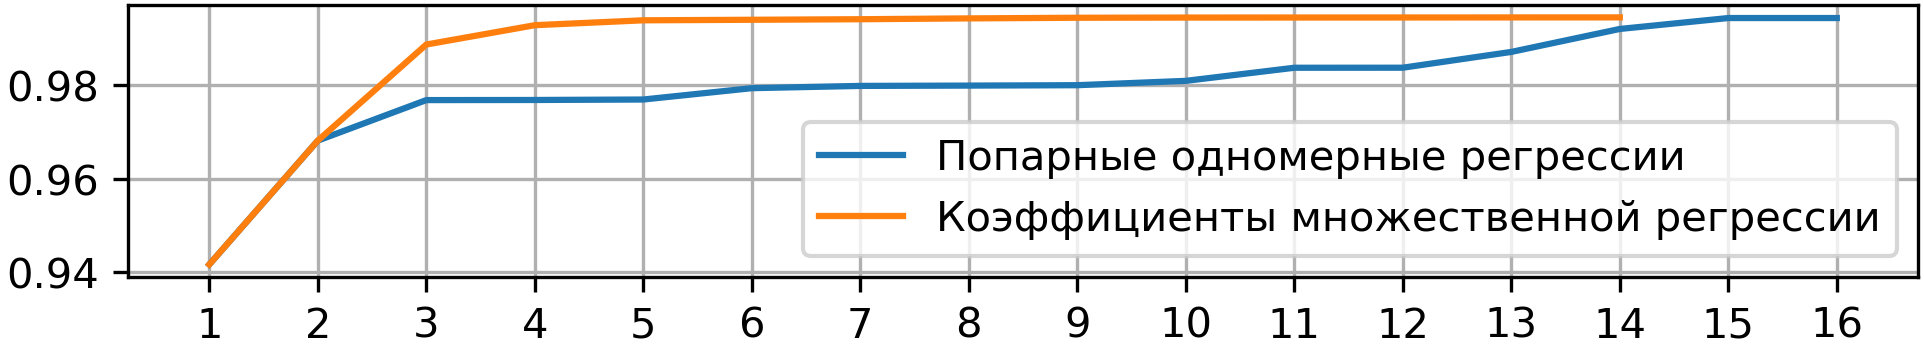
\includegraphics[width=0.8\linewidth]{pictures/Сравнение алгоритмов}
    \\
	\caption{Кривые оценок для двух алгоритмов}
\end{figure}

Алгоритм \texttt{a1} приближается к значениям алгоритма \texttt{a2}, которые получаются после добавления первых трех по значимости признаков,  лишь после добавления 14 признаков.

\section{Выводы и замечания}


Разумеется, алгоритм \texttt{a2}, построенный на коэффициентах множественной регрессии, эффективнее алгоритма \texttt{a1}, построенного на попарных одномерных регрессиях. Однако у обоих алгоритмов есть свои плюсы, и есть свои минусы.

\subsection{Попарные одномерные регрессии}

Очевидный минус — он не столь эффективно выделяет действительно значимые признаки по сравнению со своим конкурентом. Но есть и плюс: его можно использовать «вслепую», не апеллируя к семантике признаков и знанию предметной области.

\subsection{Коэффициенты множественной регрессии}

Очевидный плюс — он возвращает меньшее (причем, значительно меньшее по сравнению со своим конкурентом) число значимых признаков, за счет которых добивается максимально возможного результата. Но есть и минус: если в данных зашита мультиколлинеарность, он не справляется со своей задачей и требует вмешательства аналитика, представляющего семантику признаков и знающего предметную область.

В целом можно рекомендовать к использованию оба метода. Каждый из них может найти свое применение в зависимости от конкретной ситуации и специфики данных.

\section{Литература}


\begin{enumerate}
	\item Хейдт М. Изучаем Pandas / М. Хейдт;  — Москва: ДМК Пресс, 2018. — 438 с.
	\item Бурков А. Машинное обучение без лишних слов / А. Бурков;  — СПб: Питер, 2020. — 192 с.
	\item Вьюгин, В. В. Математические основы теории машинного обучения и прогнозирования / В. В. Вьюгин; — М.: МЦИМО. — 2013. — 387~с. 
	\item Бринк Х. Машинное обучение / Х. Бринк, Дж. Ричардс, М. Феверолф  — СПб.: Питер, 2017. — 336 с.
	\item Кузнецова И.С., Белозерских А.В. Проблемы мультиколлинеарности в регрессионных моделях / Актуальные направления научных исследований XXI века: теория и практика. 2015. Т. 3. № 8–-3 (19–-3). С. 308–-312.
	\item Орлова И.В. Подход к решению проблемы мультиколлинеарности с помощью преобразования переменных / Фундаментальные исследования. 2019. № 5. С. 78--84.
\end{enumerate}


\end{document}
